

\chapter{Public Key Encryption}
	
	\begin{itemize}
		\item Key Exchange requires interaction
		\item To send mail we don t want to interact with the receiver
		\item In private key encryption same key $K$ is used to encrypt and decrypt
		\item In public key encryption, we have a dedicated public key $pk$ which is used to encrypt
		\item As the name suggests, this key is made public
		\item Anyone can encrypt using $pk$
		\item A secret key $sk$ to decrypt
	\end{itemize}
	\begin{center}
		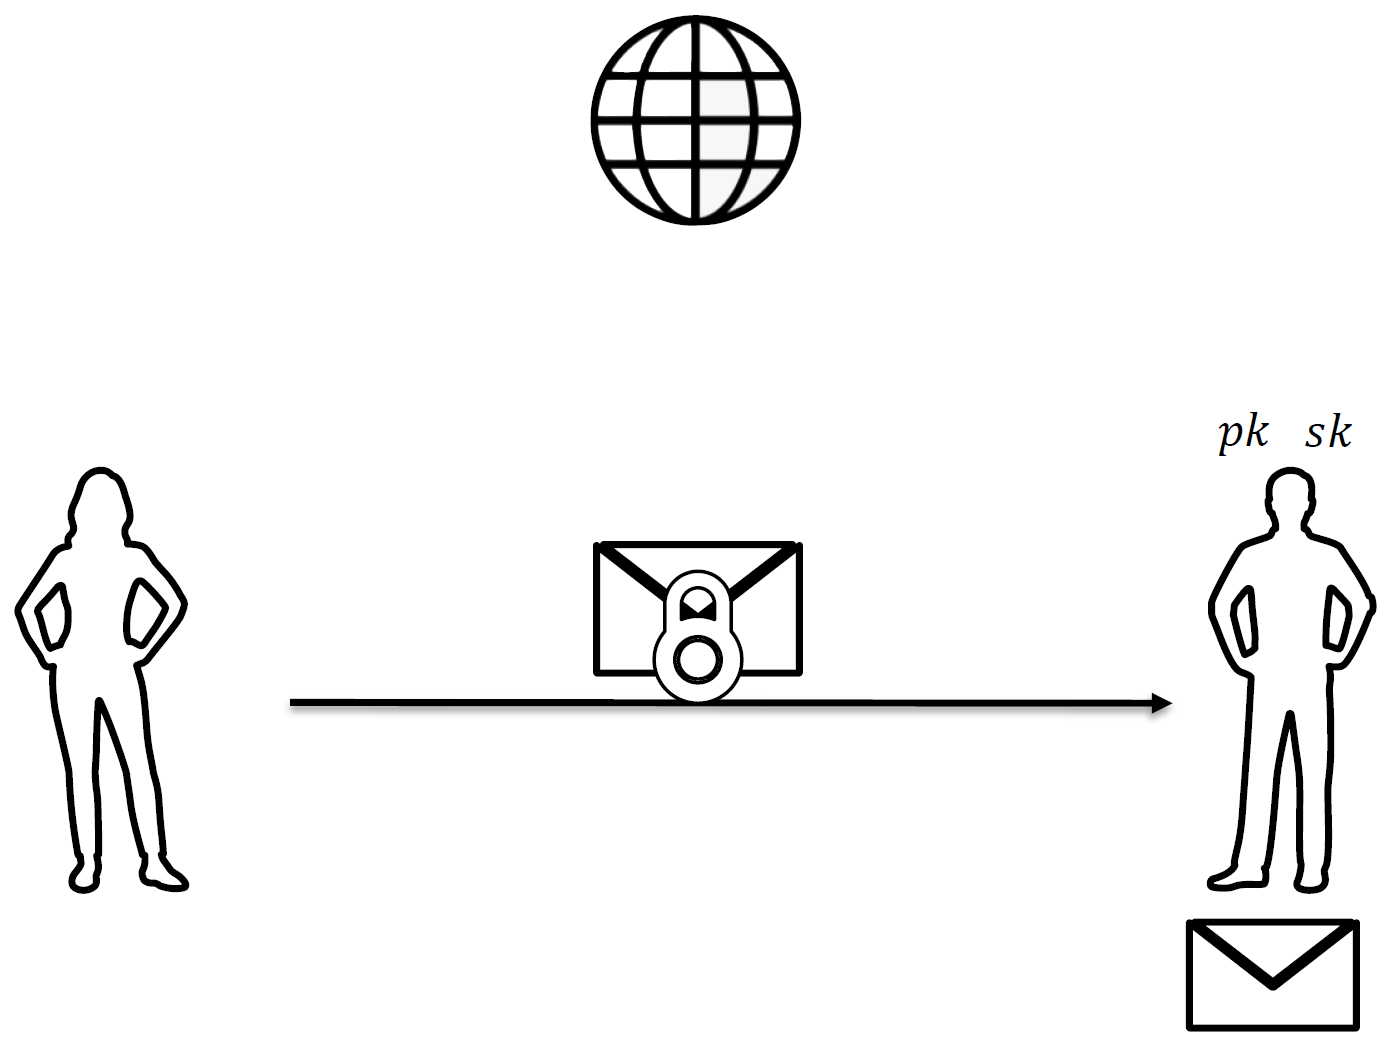
\includegraphics[width=120mm]{Graphics/Public Key Encryption/pke1.png}
	\end{center}
			
\section{Encryption Schemes}
	\textbf{Syntax:} A public key encryption scheme consists of three PPT algorithms: $(KeyGen,Enc,Dec)$
	\begin{itemize}
		\item $KeyGen(1^{\lambda})$: A randomized algorithm which takes as input the security parameter $1^{\lambda}$ (encoded in unary) 
		and outputs a pair of \textbf{public} and \textbf{secret} keys $(pk,sk)$
		\item $Enc(pk,m)$: A randomized algorithm which takes a public key $pk$ and message $m$ as input and outputs a ciphertext $c$
		\item $Dec(sk,c)$: A deterministic algorithm which takes as a secret key $sk$ and a ciphertext $c$ as input and outputs a message $m$
	\end{itemize}
	\textbf{Correctness:} It holds for all $\lambda \in \mathbb{N}$ and all messages $m$ that $Pr[Dec(sk,Enc(pk,m))=m]=1$, where $(pk,sk) \leftarrow KeyGen(1^{\lambda})$

\section{First Proposal}
	\begin{itemize}
		\item Rivest, Shamir and Adleman provided the first proposal of a public key encryption scheme 1978
		\item Commonly referred to as \textbf{Textbook RSA} today
		\begin{itemize}
			\item $KeyGen(1^{\lambda})$: Choose two random $\lambda$-bit primes $P,Q$, set $N \leftarrow P \cdot Q$ and $\Phi(N) = (P-1) \cdot (Q-1)$, 
			choose random $e \leftarrow_{\$} \mathbb{Z}_{\Phi(N)}$ with $gcd(e,\Phi(N)) = 1$ and compute $d$ s.t. $ ed \equiv 1 \ mod\ \Phi(N)$. 
			Output $pk \leftarrow (N,e)$ and $sk \leftarrow (N,d)$.
			\item $Enc(pk,m \in \mathbb{Z}_N)$: Compute and output $c \leftarrow m^e \ mod\ N$.
			\item $Dec(sk,c)$: Compute and output $m \leftarrow c^d \ mod\ N$.
		\end{itemize}
	\end{itemize}
	\textbf{Correctness:} 
	\begin{align*}
		Dec(sk,Enc(pk,m)) &= m^{e \cdot d} \ mod\ N\\
		&= m^{1 + b \cdot \Phi(N)} \ mod\ N\\
		&= m \cdot \underbrace{m^{b \cdot \Phi(N)}}_{=1} \ mod\ N
	\end{align*}

\section{What about Security?}
	\begin{itemize}
		\item Many problems with textbook RSA as encryption scheme
		\item Main problem: Encryption is deterministic
		\begin{itemize}
			\item We can test whether a ciphertext $c$ encrypts a message $m$ by testing whether $c = Enc(pk,m)$
		\end{itemize}
		\item Many other problems (features?) with textbook RSA:
		\begin{itemize}
			\item E.g. if $c = Enc(pk,m)$, then $2^e \cdot c \ mod \ N = Enc(pk,2m)$
		\end{itemize}
	\end{itemize}

\section{Defining Security}
	\begin{itemize}
		\item We will define IND-CPA security of public key encryption analogously to IND-CPA security of private key encryption
		\item Adversary $\mathcal{A}$ additionally gets public key $pk$ as input
		\item Bonus: We don t need encryption oracle as $\mathcal{A}$ can encrypt by itself using $pk$
	\end{itemize}

\newpage

\begin{definition}[IND-CPA-secure]
	An encryption scheme $(KeyGen,Enc,Dec)$ is IND-CPA\textbf{-secure}, if it holds for \textbf{PPT-secure $\mathcal{A}$} 
	there exists a negligible function $v$ s.t. for all $\lambda \in \mathcal{N}$
	$$Pr[IND-CPA_{\mathcal{A}} = 1] < \frac{1}{2} + v(\lambda)$$
\end{definition}
\begin{center}
	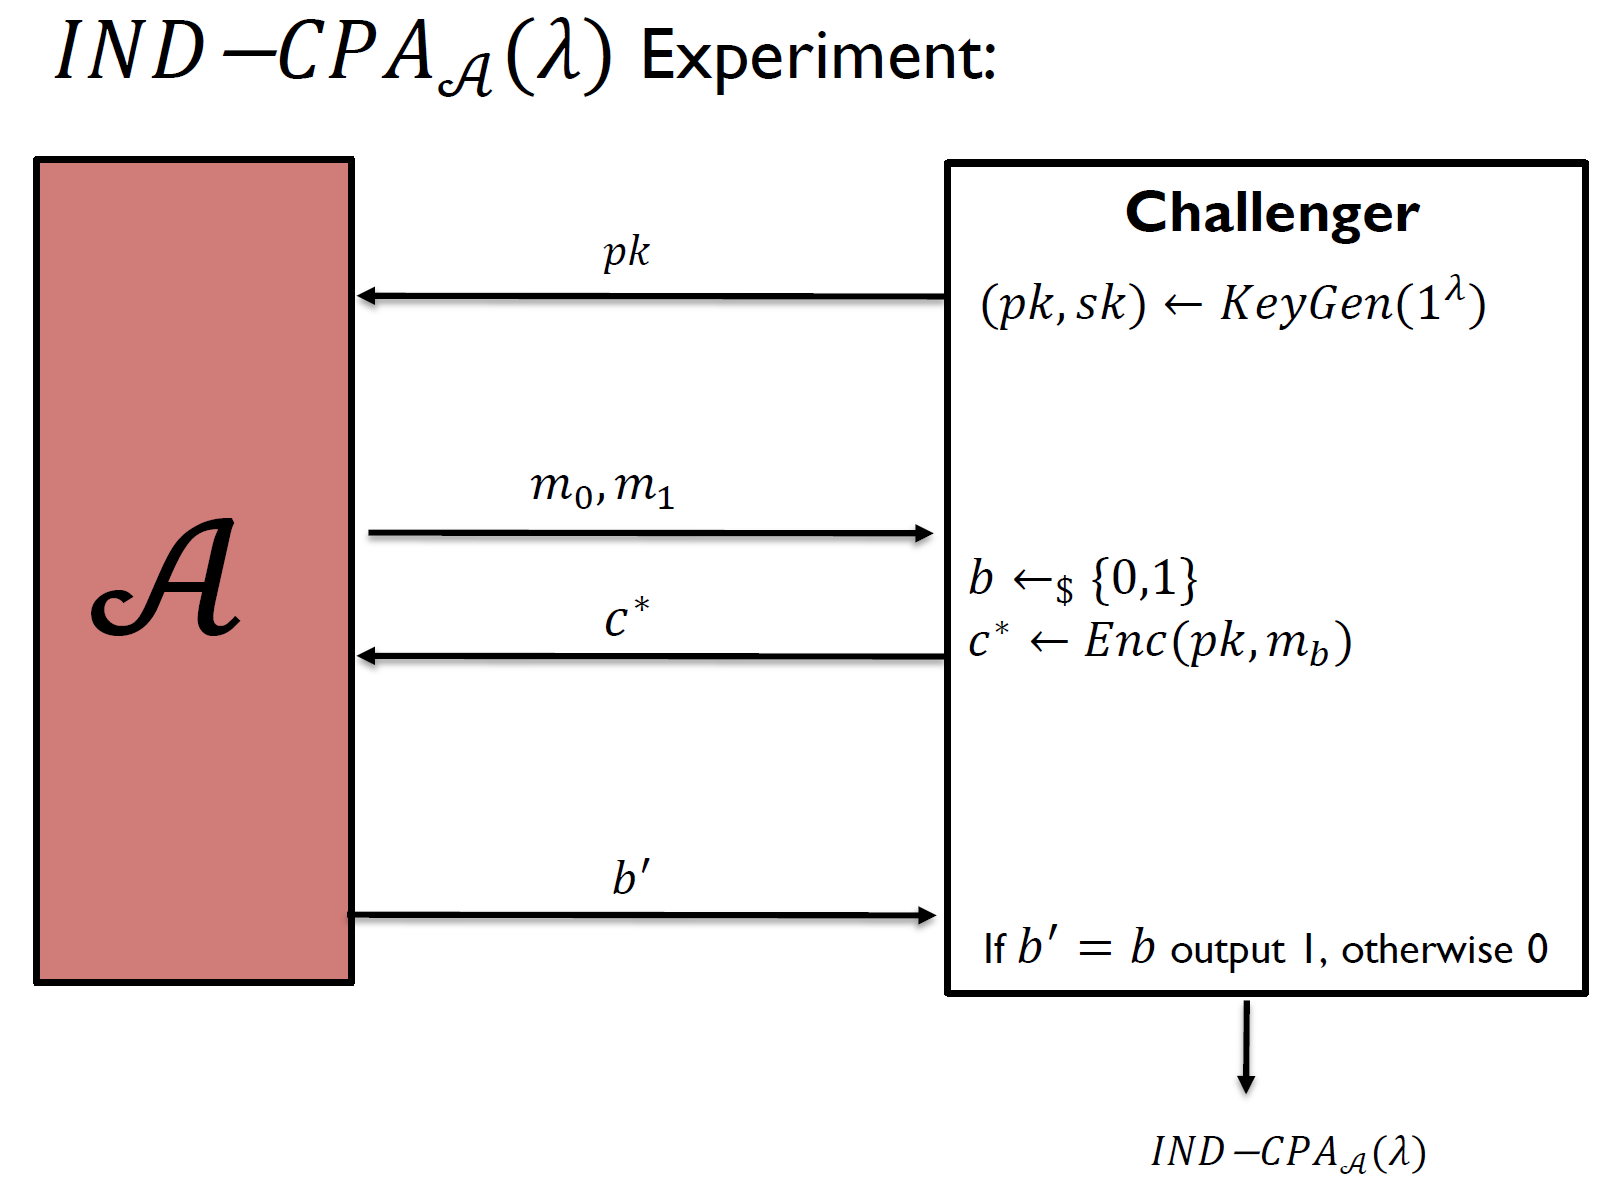
\includegraphics[width=140mm]{Graphics/Public Key Encryption/pke2.png}
\end{center}

\section{The ElGamal Cryptosystem}
	\begin{itemize}
		\item We will now construct an encryption scheme based on the Diffie-Hellman key exchange
		\item The ElGamal encryption scheme $(KeyGen,Enc,Dec)$ is given as follows
		\begin{itemize}
			\item $KeyGen(1^{\lambda})$:
			\begin{itemize}
				\item Generate cryptographic group $\mathbb{G}$ of prime order $p \approx 2^{\lambda}$ with generator $g$
				\item Choose $x \leftarrow_{\$} \mathbb{Z}_p$ uniformly at random and set $h \leftarrow g^x$
				\item Output $pk \leftarrow (g,h)$ and $sk \leftarrow x$
				\item (implicity assume that $pk$ include description of $\mathbb{G}$ and $p$)
			\end{itemize}
			\item $Enc(pk=(g,h),m \in \mathbb{G})$: Choose $y \leftarrow_{\$} \mathbb{Z}_p$, compute and output $c \leftarrow (g^y,h^y \cdot m)$
			\item $Dec(sk=x,c=(c_1,c_2))$: Compute and output $m \leftarrow c_2 \cdot c_1^{-x}$
		\end{itemize}
	\end{itemize}
	\textbf{Correctness:} $(c_1,c_2) = Enc(pk,m)$, $pk = (g,h=g^x)$, $sk=x$, $c_1 = g^y$, $c_2 = h^y \cdot m$\\
		$\Rightarrow Dec(sk=x,(c_1,c_2)) = c_2 \cdot c_1^{-x} = h^y \cdot m \cdot (g^y)^{-x} = g^{x \cdot y} \cdot m \cdot g^{-x \cdot y} = m$

\begin{theorem}
	\begin{itemize}\label{thm8.2}\ 
		\item Assume that the DDH-assumption holds in the group $\mathbb{G}$
		\item Then the ElGamal encryption scheme $(KeyGen,Enc,Dec)$ is IND-CPA secure
	\end{itemize}
\end{theorem}
\begin{proof}
	Assume towards contradiction there exists a PPT adversary $\mathcal{A}$ and a non-negligible $\epsilon$ s.t. $Pr[IND-CPA_{\mathcal{A}}(\lambda)=1] \geq \frac{1}{2} + \epsilon$\\
	\underline{Show:} This implies a PPT-distinguisher $\mathcal{D}$ against DDH, contradicting the DDH assumption.
\begin{center}
	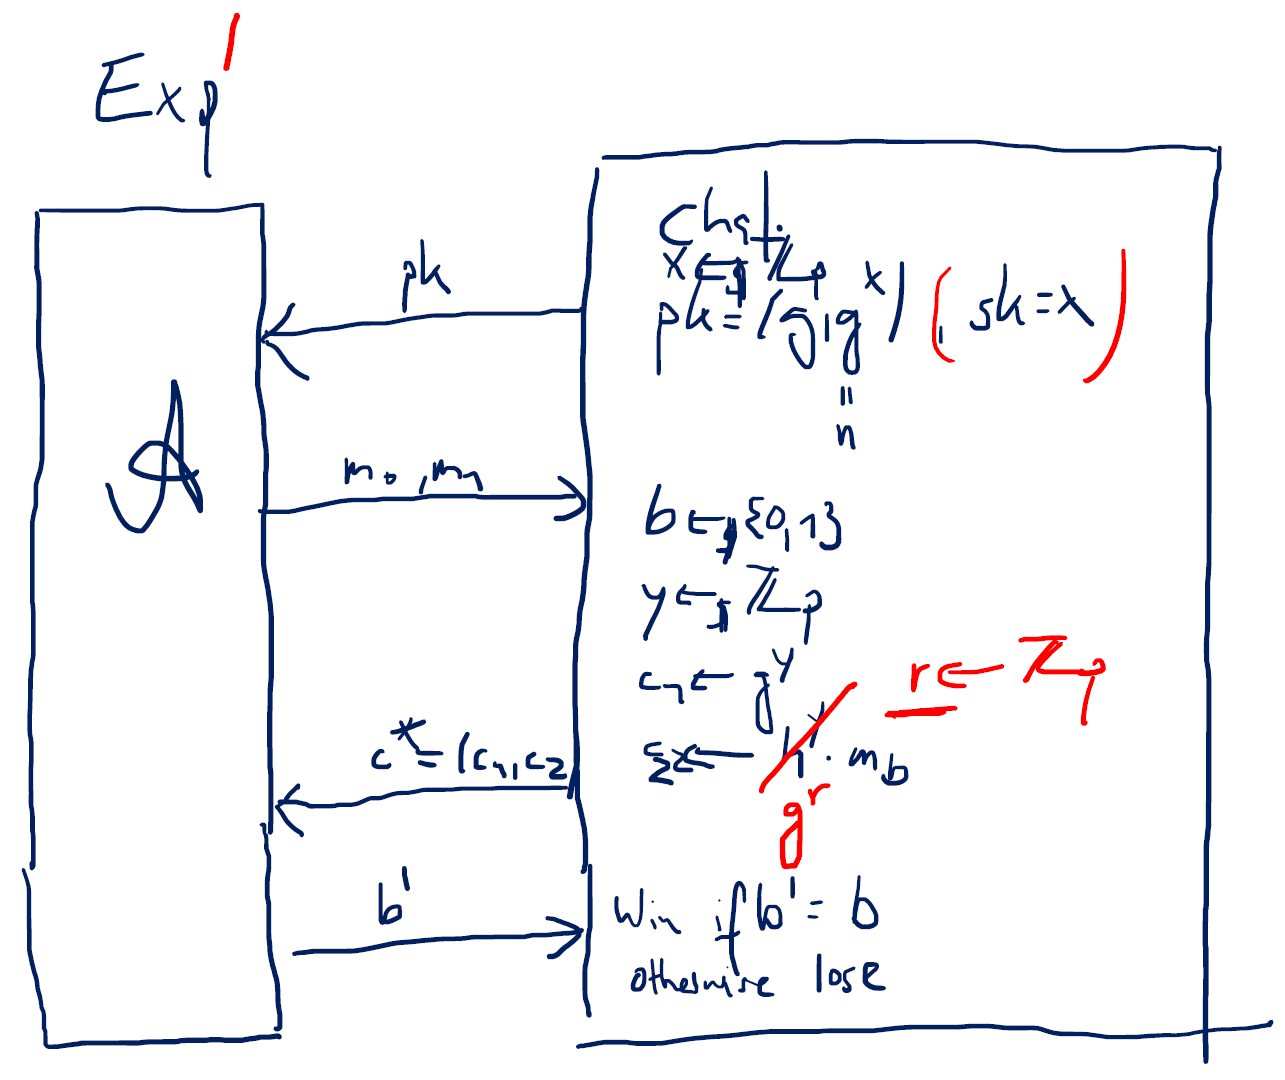
\includegraphics[width=120mm]{Graphics/Public Key Encryption/pke3.png}
\end{center}

$g^r$ is uniform in $\mathbb{G}$ $\Rightarrow$ $Pr[Exp'=1] = \frac{1}{2}$\\

Construct PPT-distinguisher $\mathcal{D}$ against DDH

\begin{center}
	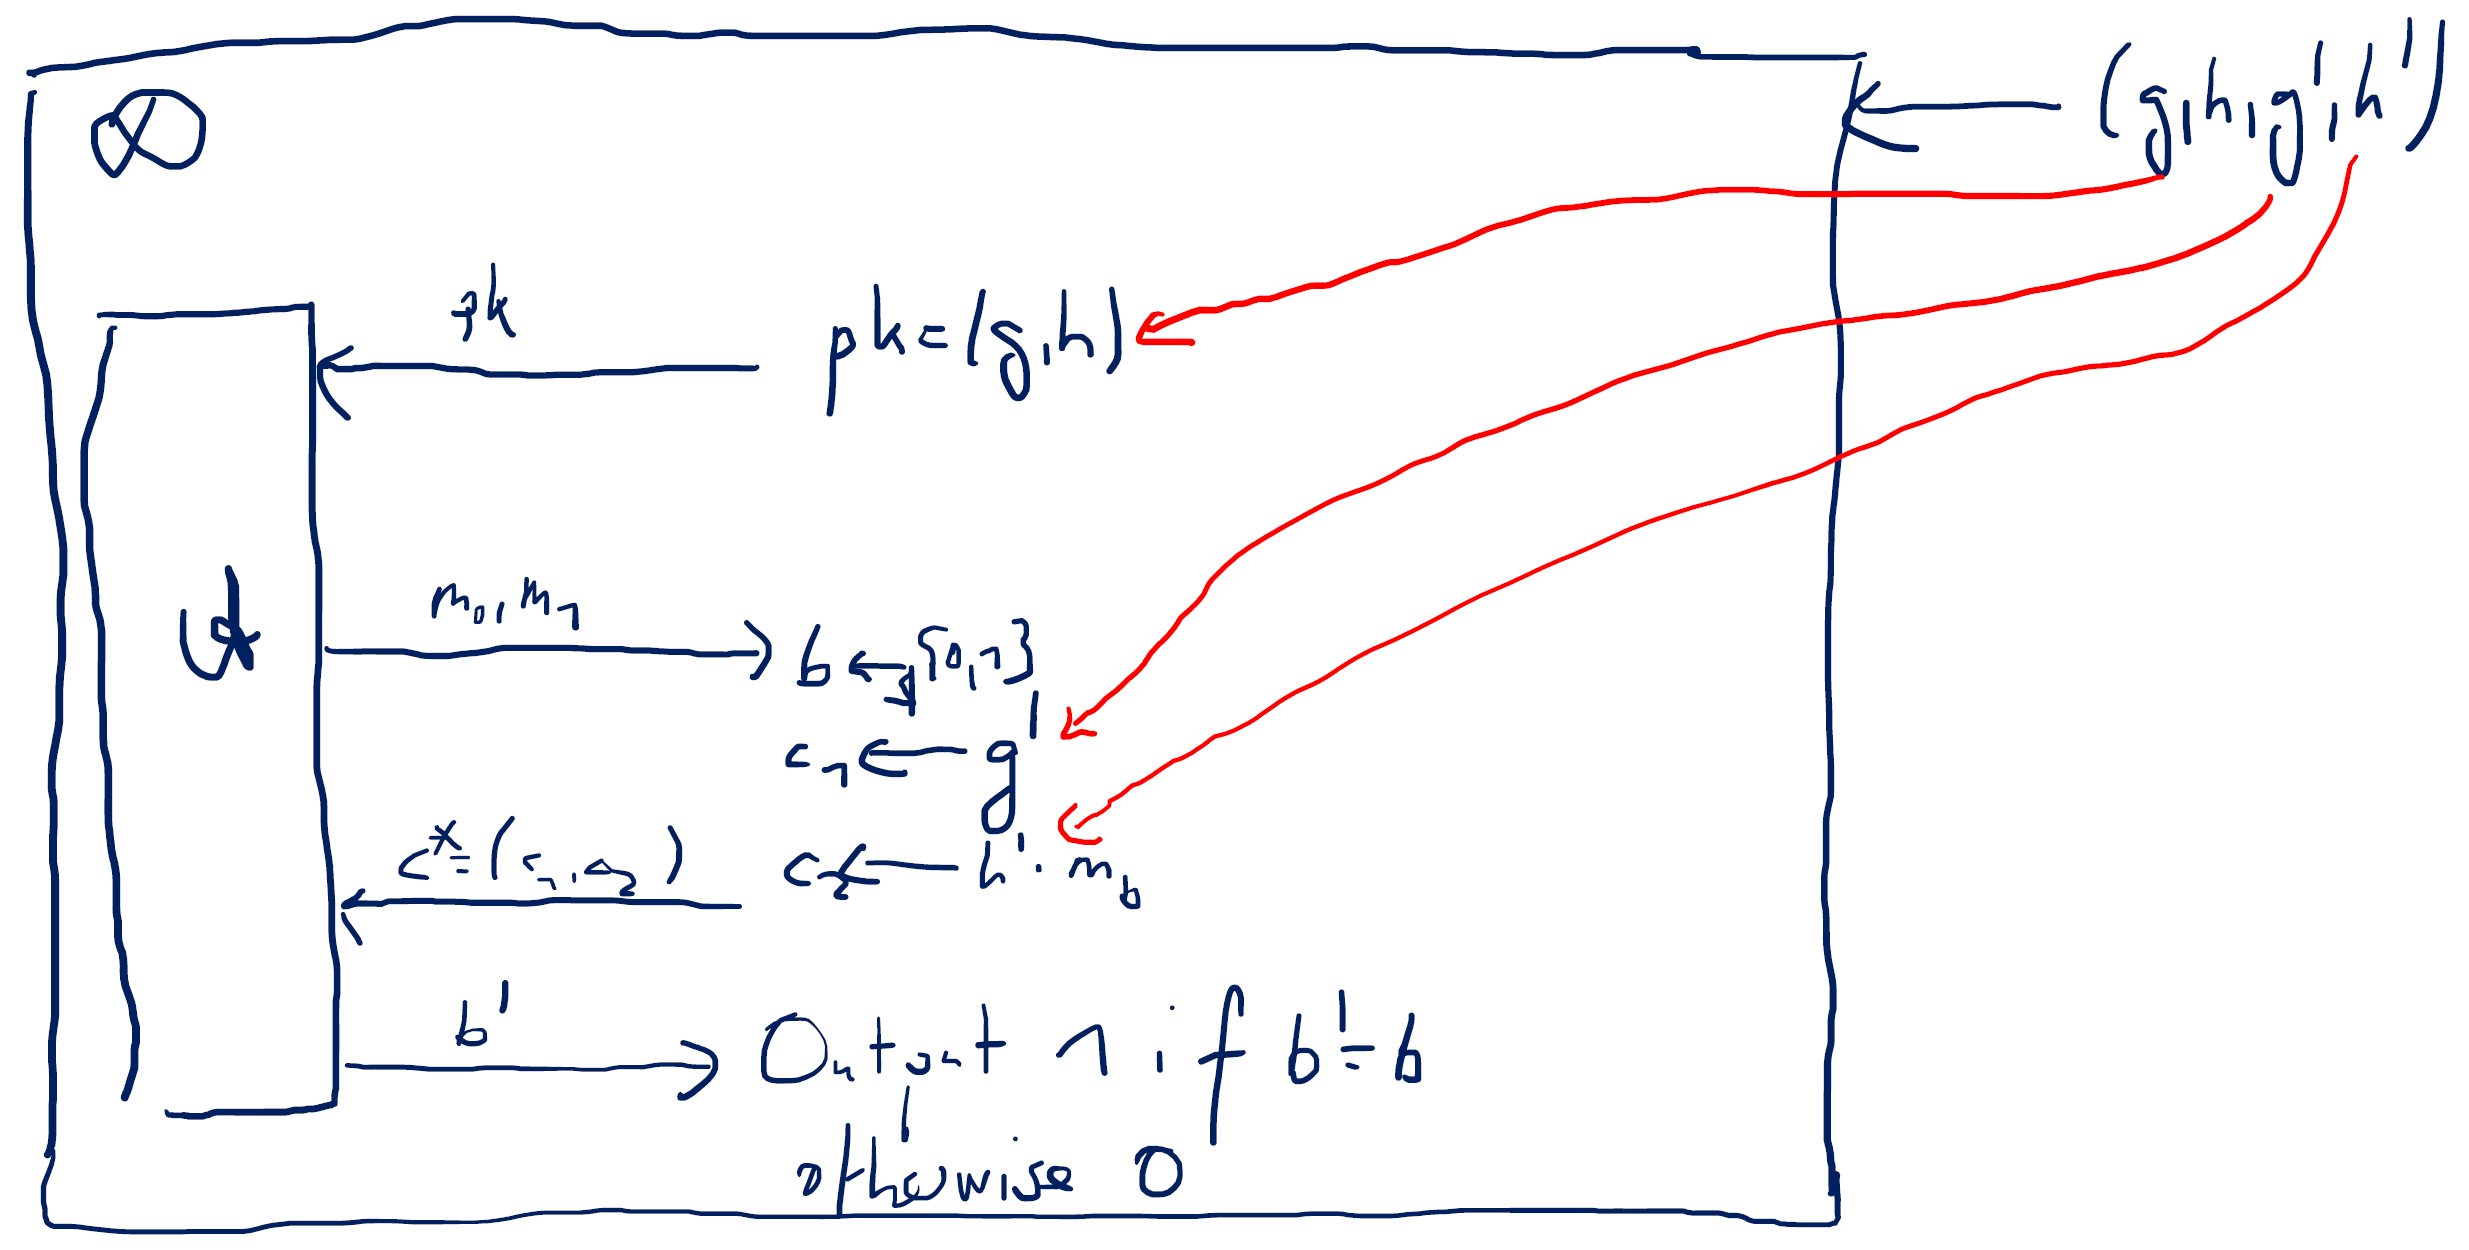
\includegraphics[width=140mm]{Graphics/Public Key Encryption/pke4.png}
\end{center}
	\textbf{\underline{Case 1:}}
		$(g,h,g',h')=(g,g^x,g^y,g^{xy})$, $x,y \leftarrow_{\$} \mathbb{Z}_p$\\
		$\Rightarrow$ In this case $\mathcal{D}$ faithfully simulates the IND-CPA experiment\\
		$h=g^x$, $c_1 = g^y$, $c_2 = g^{xy} \cdot m_b = h^y \cdot m_b$\\
		$\Rightarrow$ $Pr[\mathcal{D}(g,g^x,g^y,g^{xy})=1] = Pr[IND-CPA_{\mathcal{A}}(\lambda)=1] \geq \frac{1}{2} + \epsilon$\\\\
	\textbf{\underline{Case 2:}}
		$(g,h,g',h')=(g,g^x,g^y,g^{r})$, $x,y,r \leftarrow_{\$} \mathbb{Z}_p$\\
		$\Rightarrow$ In this case $\mathcal{D}$ faithfully simulates $Exp'$\\
		$\Rightarrow$ $Pr[\mathcal{D}(g,g^x,g^y,g^{r})=1] = Pr[Exp'=1] = \frac{1}{2}$\\
		$\Rightarrow$ $|Pr[\mathcal{D}(g,g^x,g^y,g^{xy})=1]-Pr[\mathcal{D}(g,g^x,g^y,g^{r})=1]| \geq \frac{1}{2} + \epsilon - \frac{1}{2} = \epsilon$ which is non-negligible!\\
		$\Rightarrow$ $\mathcal{D}$ distinguishes DDH-problem with advantage $\epsilon$
\end{proof}

\section{Summary}
	\begin{itemize}
		\item Public key encryption allows for secure communication without prior interaction
		\item The textbook RSA scheme is not an encryption scheme by modern standards (...but a useful building block)
		\item The standard security notion of public key encryption is IND CPA security, adapted from the private key definition
		\item The ElGamal encryption scheme is IND CPA secure under the Decisional Diffie Hellman (DDH) assumption
	\end{itemize}


